\documentclass[12pt, letterpaper]{article}
\usepackage{graphicx} % Required for inserting images
\usepackage{hyperref}
\usepackage{listings}
\usepackage{amssymb}
\usepackage{amsmath}
\usepackage[english]{babel}
\usepackage{nicefrac, xfrac}
\usepackage{mathtools}
\usepackage[table,xcdraw]{xcolor}
\definecolor{light-gray}{gray}{0.95}
\definecolor{sap}{RGB}{130, 36, 51}
\definecolor{lg}{RGB}{102, 161, 95}
\usepackage[paper=a4paper,left=20mm,right=20mm,bottom=25mm,top=25mm]{geometry}
\newcommand{\code}[1]{\colorbox{light-gray}{\texttt{#1}}}
\newcommand{\shelll}[1]{\colorbox{black}{\textcolor{white}{\texttt{#1}}}}
\newcommand{\shell}[1]{\colorbox{black}{\textcolor{white}{\texttt{casufrost@debian:$\sim$\$ #1}}}}
\newcommand{\codee}[1]{\colorbox{white}{\texttt{#1}}}
\newcommand{\acc}{\\\hphantom{}\\}
\newcommand{\dete}{{\rightarrow}}
\newcommand{\fdot}{{\(\bullet\) }}
\newcommand{\boxedMath}[1]{\begin{tabular}{|c|}\hline \texttt{#1} \\ \hline\end{tabular} :}
\title{Sistemi Operativi 2}
\author{Marco Casu}
\date{\vspace{-5ex}}
\begin{document}



\maketitle
\begin{figure}[h]
    \centering{
    
\includegraphics[width=1\textwidth ]{images/cop.jpg}
    }
\end{figure}
\newpage 
\tableofcontents
\newpage
\section{Introduzione}
\subsection{Breve Panoramica su Unix}
Moltissimi sistemi operativi moderni, come \textit{MacOs}, \textit{Linux}, e molti altri, sono basati 
su \textbf{\textit{Unix}}, un sistema operativo il cui sviluppo cominciò nel lontano 1965. Inizialmente implmenetato 
totalmente in assembly, e limitato esclusivamente ad un tipo di architettura, si decise di costruire dei linguaggi 
di programmazione di più alto livello per garantire la portabilità, le versioni di Unix nei linguaggi \textit{B} e 
\textit{C} permisero di portare Unix su diverse CPU.\acc 
Venne distribuito con codice sorgente a centri di ricerca ed università, si diffuse rapidamente e nacquero diverse 
versioni. Le caratteristiche principali di un OS basato su Unix sono le seguenti: \begin{itemize}
    \item Supporta più utenti e la multiprogrammazione 
    \item Il file system ha un organizzazione gerarchica 
    \item Ha un kernel rappresentante il cuore del sistema 
    \item Si interagisce col kernel tramiite le chiamate di sistema
    \item Ha una \textit{shell} (si vedrà in seguito)
    \item È modulare e fornisce ambienti di programmazione
\end{itemize}
È composto da una serie di programmi limitati che eseguono molto bene un compito specifico, presentano un output 
minimale, sono detti "silenziosi", e lavori più complessi possono essere svolti componendo ed articolando diversi programmi 
semplici. I programmi solitamente manipolano file di testo (interpretabili dall'uomo secondo la codifica ASCII) e non file 
binari. Qualsiasi risorsa può essere vista come file o come processo.
\subsection{La Shell}
La \textbf{Shell} non è altro che un programma che esegue dei comandi, che possono essere scritti sul 
terminale, esistono vari tipi di shell, come quella denominata \textit{bash}. La bash scrive il cosiddetto 
\textit{prompt}, ossia una dicitura che indica che il terminale è in attesa di ricevere comandi, molto spesso è 
costituito dal nome dell'utente, il nome del computer, ed il percorso della directory nella quale è aperto il 
terminale.\acc
\shelll{nomeutente@nomemacchina:$\sim$\$} \textit{in attesa di ricevere comandi}
\acc 
Ogni \textbf{comando} seguirà il seguente template : Prima il nome del comando, poi le varie opzioni, e poi gli argomenti 
del comando, ci deve essere almeno un argomento obbligatorio, e zero o più argomenti opzionali, gli argomenti vanno 
separati da un carattere se indicato. \textit{Esempio} :\acc 
\shell{ps -p \$\$ -ocmd -h}
\acc 
Uno dei comandi fondamentali è \code{man}, e sta per \textit{manuale}, è un comando fondamentale che fornisce 
le informazioni più autorevoli possibile riguardo un comando, basta chiamarlo, dando come argomento appunto, il 
nome di un comando, e fornirà una lista dettagliata di tutte le opzioni ad esso correlato.\acc 
\shell{man ps} produce il seguente output : \begin{center}
    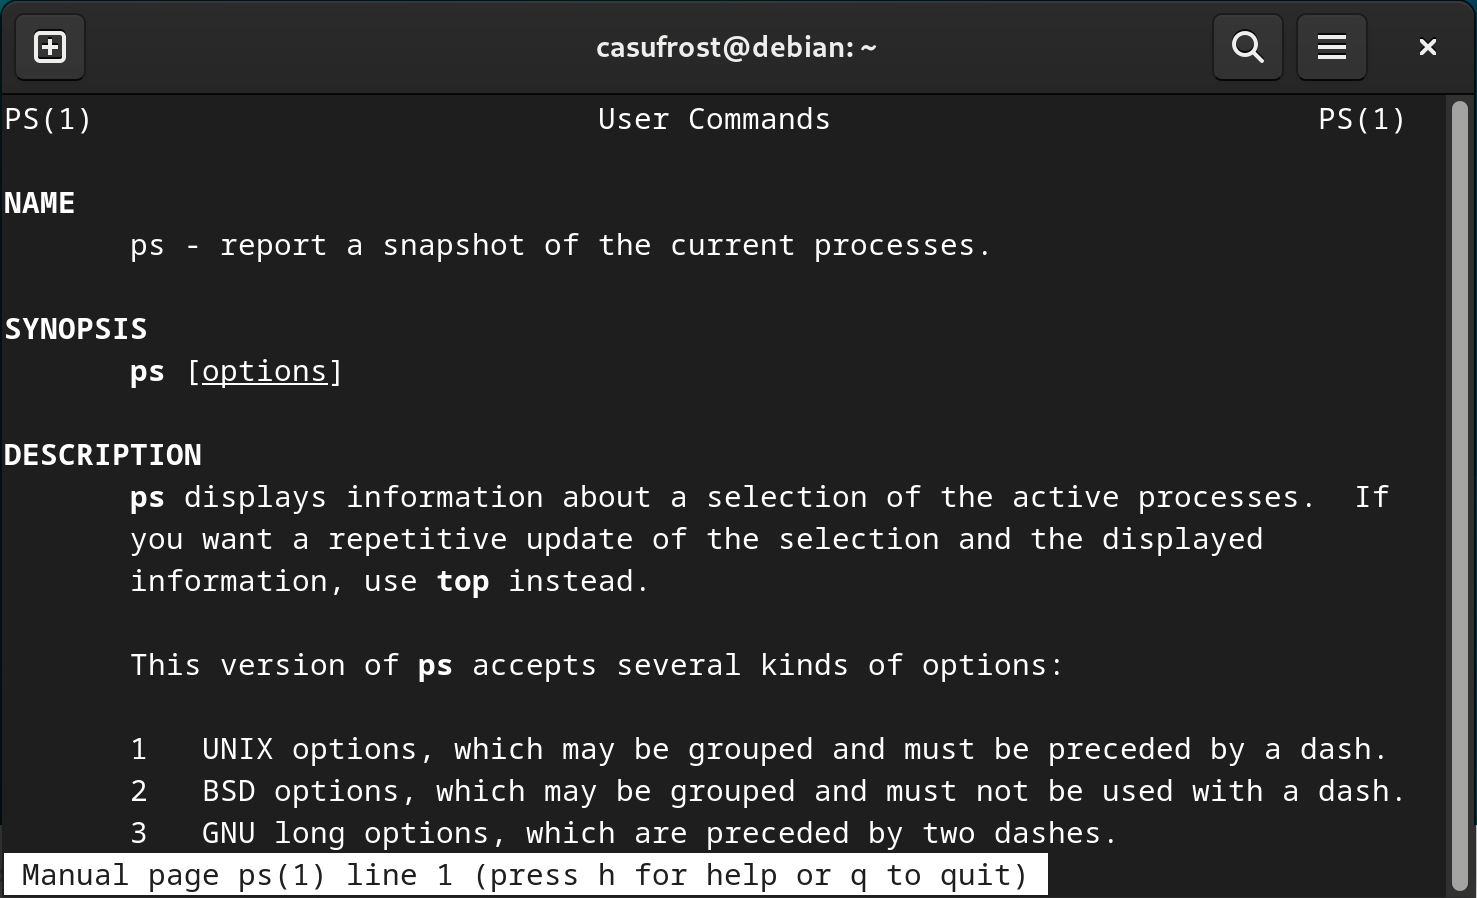
\includegraphics[width=0.7\textwidth ]{images/manPs.png}
\end{center}
Consultando il manuale è possibile capire come utilizzare i comandi fondamentali : 
\begin{itemize}
    \item \shelll{ps} - Mostra le informazioni dei processi attualmente in esecuzione.
    \item \shelll{ls} - Mostra una lista delle risorse contenute in una directory.
    \item \shelll{cp} - Copia file e directory.
\end{itemize}
Analizziamo il comando di esempio scritto in precedenza, ossia: \acc\shell{ps -p \$\$ -ocmd -h} tale comando 
mostra i processi attualmente in esecuzione, l'opzione serve a selezionare il processo in base al suo 
PID, e prede come parametro \code{\$\$}, ossia il codice identificativo del processo bash. \acc Il comando mostra 
varie informazioni, come il PID del processo ed il nome, L'opzione \code{-o} serve a selezionare solo uno dei 
parametri del processo, in questo caso prende come argomento \code{cmd} e seleziona quindi solo quel campo, ossia 
il nome. Si noti come in questo caso non è necessario lasciare uno spazio fra l'opzione e l'argomento. L'ultima opzione, 
ossia \code{-h}, serve a rimuovere il nome dei campi visualizzati, ci si aspetta quindi che tale comando in output 
restituirà esclusivamente il nome del processo bash : \acc 
\shell{ps -p \$\$ -ocmd -h}\\
\shelll{bash}\acc 
Un altro esempio : \acc 
\shell{ps -p \$\$}\\
\shelll{\space\space PID\space\space TTY\space\space\space\space\space\space TIME\space\space\space CMD\space}\\
\shelll{\space 3134\space pts/0\space\space\space 00:00:00\space bash}\acc 
Durante la configurazione di un sistema Unix è necessario specificare almeno un utente. Differenti utenti hanno 
differenti privilegi, l'utente \textbf{root}, o \textbf{superutente}, è predefinito in ogni sistema 
e possiede tutti i privilegi, è detto \textit{amministratore di sistema}.\acc 
Tale utente però, non può effettivamente eseguire un login ed entrare nel sistema, se necessario eseguire un 
operazione privilegiata, gli altri utenti possono acquisire temporaneamente i diritti di amministratore tramite 
il comando \shelll{sudo}, acronimo di \textit{super user do}.\acc 
Gli utenti appartengono a dei \textit{gruppi} che definiscono diversi privilegi, coloro che possono richiedere 
temporaneamente i diritti di amministratore appartengono al gruppo dei \textit{sudoers}, è possible mostrare 
a quali gruppi appartiene un utente tramite il comando \shelll{groups}.\acc 
\shelll{sudo} è un comando che prende come input un altro comando da eseguire in modalità root, esiste anche un altro 
comando chiamato \shelll{su}, e sta per \textit{substitute user}, e serve per cambiare utente, e diventare 
possibilmente amministratore, risulta comunque meno sicuro del comando \shelll{sudo}, in quanto quest'ultimo 
permette solo di eseguire un operazione in maniera privilegiata, senza rimanere nella condizione di root.
\end{document}
